\section{Módulo Telit GL865-QUAD}
\subsection{Prueba unitaria}
Para verificar que el módulo tenga un correcto funcionamiento, se probó de manera unitaria el UART del módulo Telit GL865-QUAD con un módulo FT232. La conexión entra ambos componentes se realizó de forma cruzada, es decir, que el transmisor de un dispositivo fue conectado al receptor del otro, tal como se muestra en la figura \ref{fig:ConexionUART}.

	\begin{figure}[htbp!]
		\centering
		\fbox{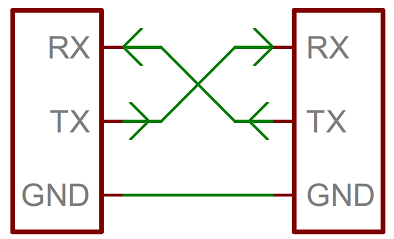
\includegraphics[width=0.4\textwidth]{AvancesPruebas/imagenes/conexion-uart.png}}
		\caption{Conexión UART de módulo GSM y FT232}
		\label{fig:ConexionUART}
	\end{figure}
	
Una vez conectado correctamente ambos módulos, se realizó la prueba de la siguiente forma:
\begin{enumerate}
	\item Se ejecutó el emulador de terminal ’PuTTY’, configurándolo para el puerto serial
	indicado, con un baudaje de 9600, transmisión de 8 bits, sin paridad con 1 bit de
	stop y sin flujo de control. La configuración realizada se muestra en la figura \ref{fig:ConfiguracionPutty}.
	\item Se ejecutaron los comandos AT básicos para probar el módulo GL865-QUAD, en ninguno de ellos
	debe aparecer un error, de lo contrario se debe revisar la conexión entre los dispositivos
	y la instalación del software necesario. Algunos de los comandos utilizados, son:
		\begin{enumerate}
			\item AT
			\item AT+GSV
			\item AT+IPR=?
			\item AT+CSQ
			\item AT+CREG? 
			\item AT+CGREG? 
			\item AT+CGNSPWR=1
			\item AT+CGNSINF=0
		\end{enumerate}	
\end{enumerate}
 
	\begin{figure}[htbp!]
		\centering
		\fbox{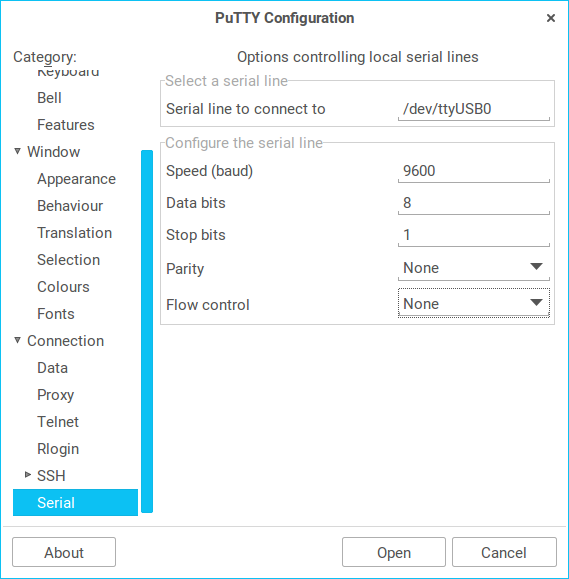
\includegraphics[width=0.5\textwidth]{AvancesPruebas/imagenes/putty.png}}
		\caption{Configuración de terminal en PuTTY}
		\label{fig:ConfiguracionPutty}
	\end{figure}
 
El resultado de los comandos ejecutados mediante la terminal de PuTTY se muestra en la figura \ref{fig:TerminalPutty}.

	\begin{figure}[htbp!]
		\centering
		\fbox{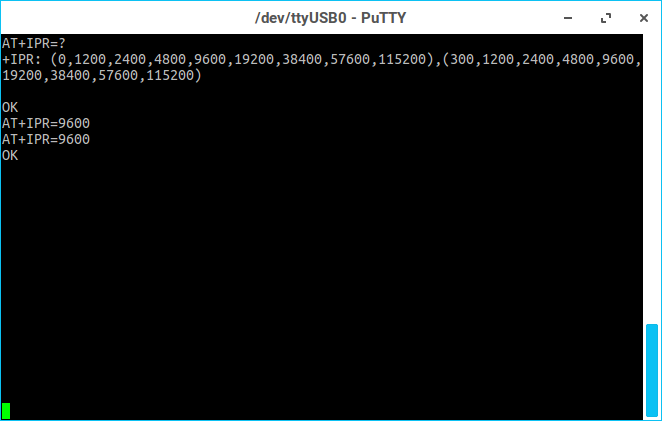
\includegraphics[width=0.6\textwidth]{AvancesPruebas/imagenes/putty_ipr.png}}
		\caption{Comandos AT en terminal de PuTTY}
		\label{fig:TerminalPutty}
	\end{figure}
\pagebreak

\subsection{Conexión con microcontrolador}
Después de asegurar el funcionamiento del módulo GSM, se realizó el programa correspondiente para la comunicación con el microcontrolador.\\

La conexión fue realizada mediante el UART2 del microcontrolador y mediante comandos AT se creó la rutina para verificar el envío de un mensaje SMS a un número de teléfono específico.

El código principal del módulo gsm se muestra a continuación:
{\small 
\begin{lstlisting}[frame=single]
; COMANDO AT PARA INICIALIZAR EL MODEM

CMD_AT: .BYTE 'A','T', 0X0D	;char CMD_AT[] = "AT\r"

; DESHABILITAR EL ECO DEL COMANDO EN LA RESPUESTA DEL MODEM

CMD_ATE0: .BYTE 'A','T','E','0',0X0D

; COMANDO AT+CPIN=1111 MANDA EL CODIGO PIN DE LA TARJETA SIM

CMD_AT_CPIN: .BYTE 'A','T','+','C','P','I','N'

.BYTE '=', '1','1','1','1',0X0D

; COMANDO AT+CMGF=1 ACTIVA EL MODO TEXTO PARA ENVIAR MENSAJES

CMD_AT_CMGF: .BYTE 'A','T','+','C','M','G','F','=','1', 0X0D

; COMANDO AT+CMGS="+525543612094" PARA DEFINIR NO DE TELEFONO

CMD_AT_CMGS: .BYTE 'A','T','+','C','M','G','S','=','"'

.BYTE '+','5','2','5','5','4','3','6','1','2','0','9','4','"',0X0D

; MENSAJE "PROBANDO GSM CLICK^z"

CMD_MSJ: .BYTE 'H','O','L','A',' ','E','L','S','I','.',' ',' ',

.BYTE 'M','S','J',' ','E','N','V','I','A','D','O'

.BYTE ' ','D','E','S','D','E',' '

.BYTE 'D','S','P','I','C','!',0X1A,0X0D

CAD_OK:         .STRING "OK"
CAD_ERROR:      .STRING "ERROR"
CAD_SIGNO_MAYOR:.STRING ">"
\end{lstlisting}
}
La conexión del módulo GSM se realizó mediante un mikrobus conectado al microcontrolador. El esquema de esta conexión, así como la conexión física se muestran en las figuras \ref{fig:ConexionAD8232} y \ref{fig:ConexionFisicaGSM} respectivamente.

	\begin{figure}[htbp!]
		\centering
		\fbox{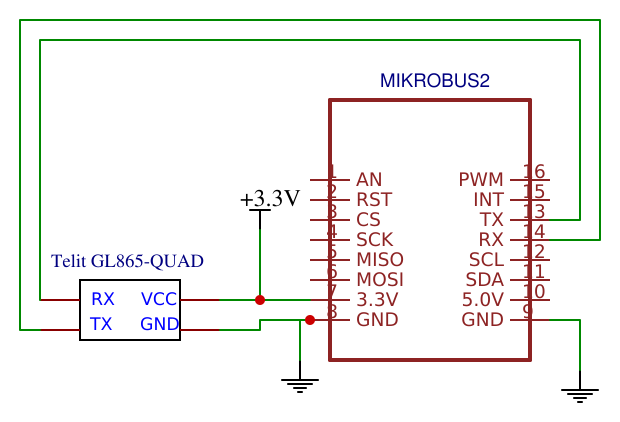
\includegraphics[width=0.7\textwidth]{AvancesPruebas/imagenes/GSMConexion.png}}
		\caption{Conexión del módulo GSM con microcontrolador}
		\label{fig:ConexionGSM}
	\end{figure}
	
	\begin{figure}[htbp!]
		\centering
		\fbox{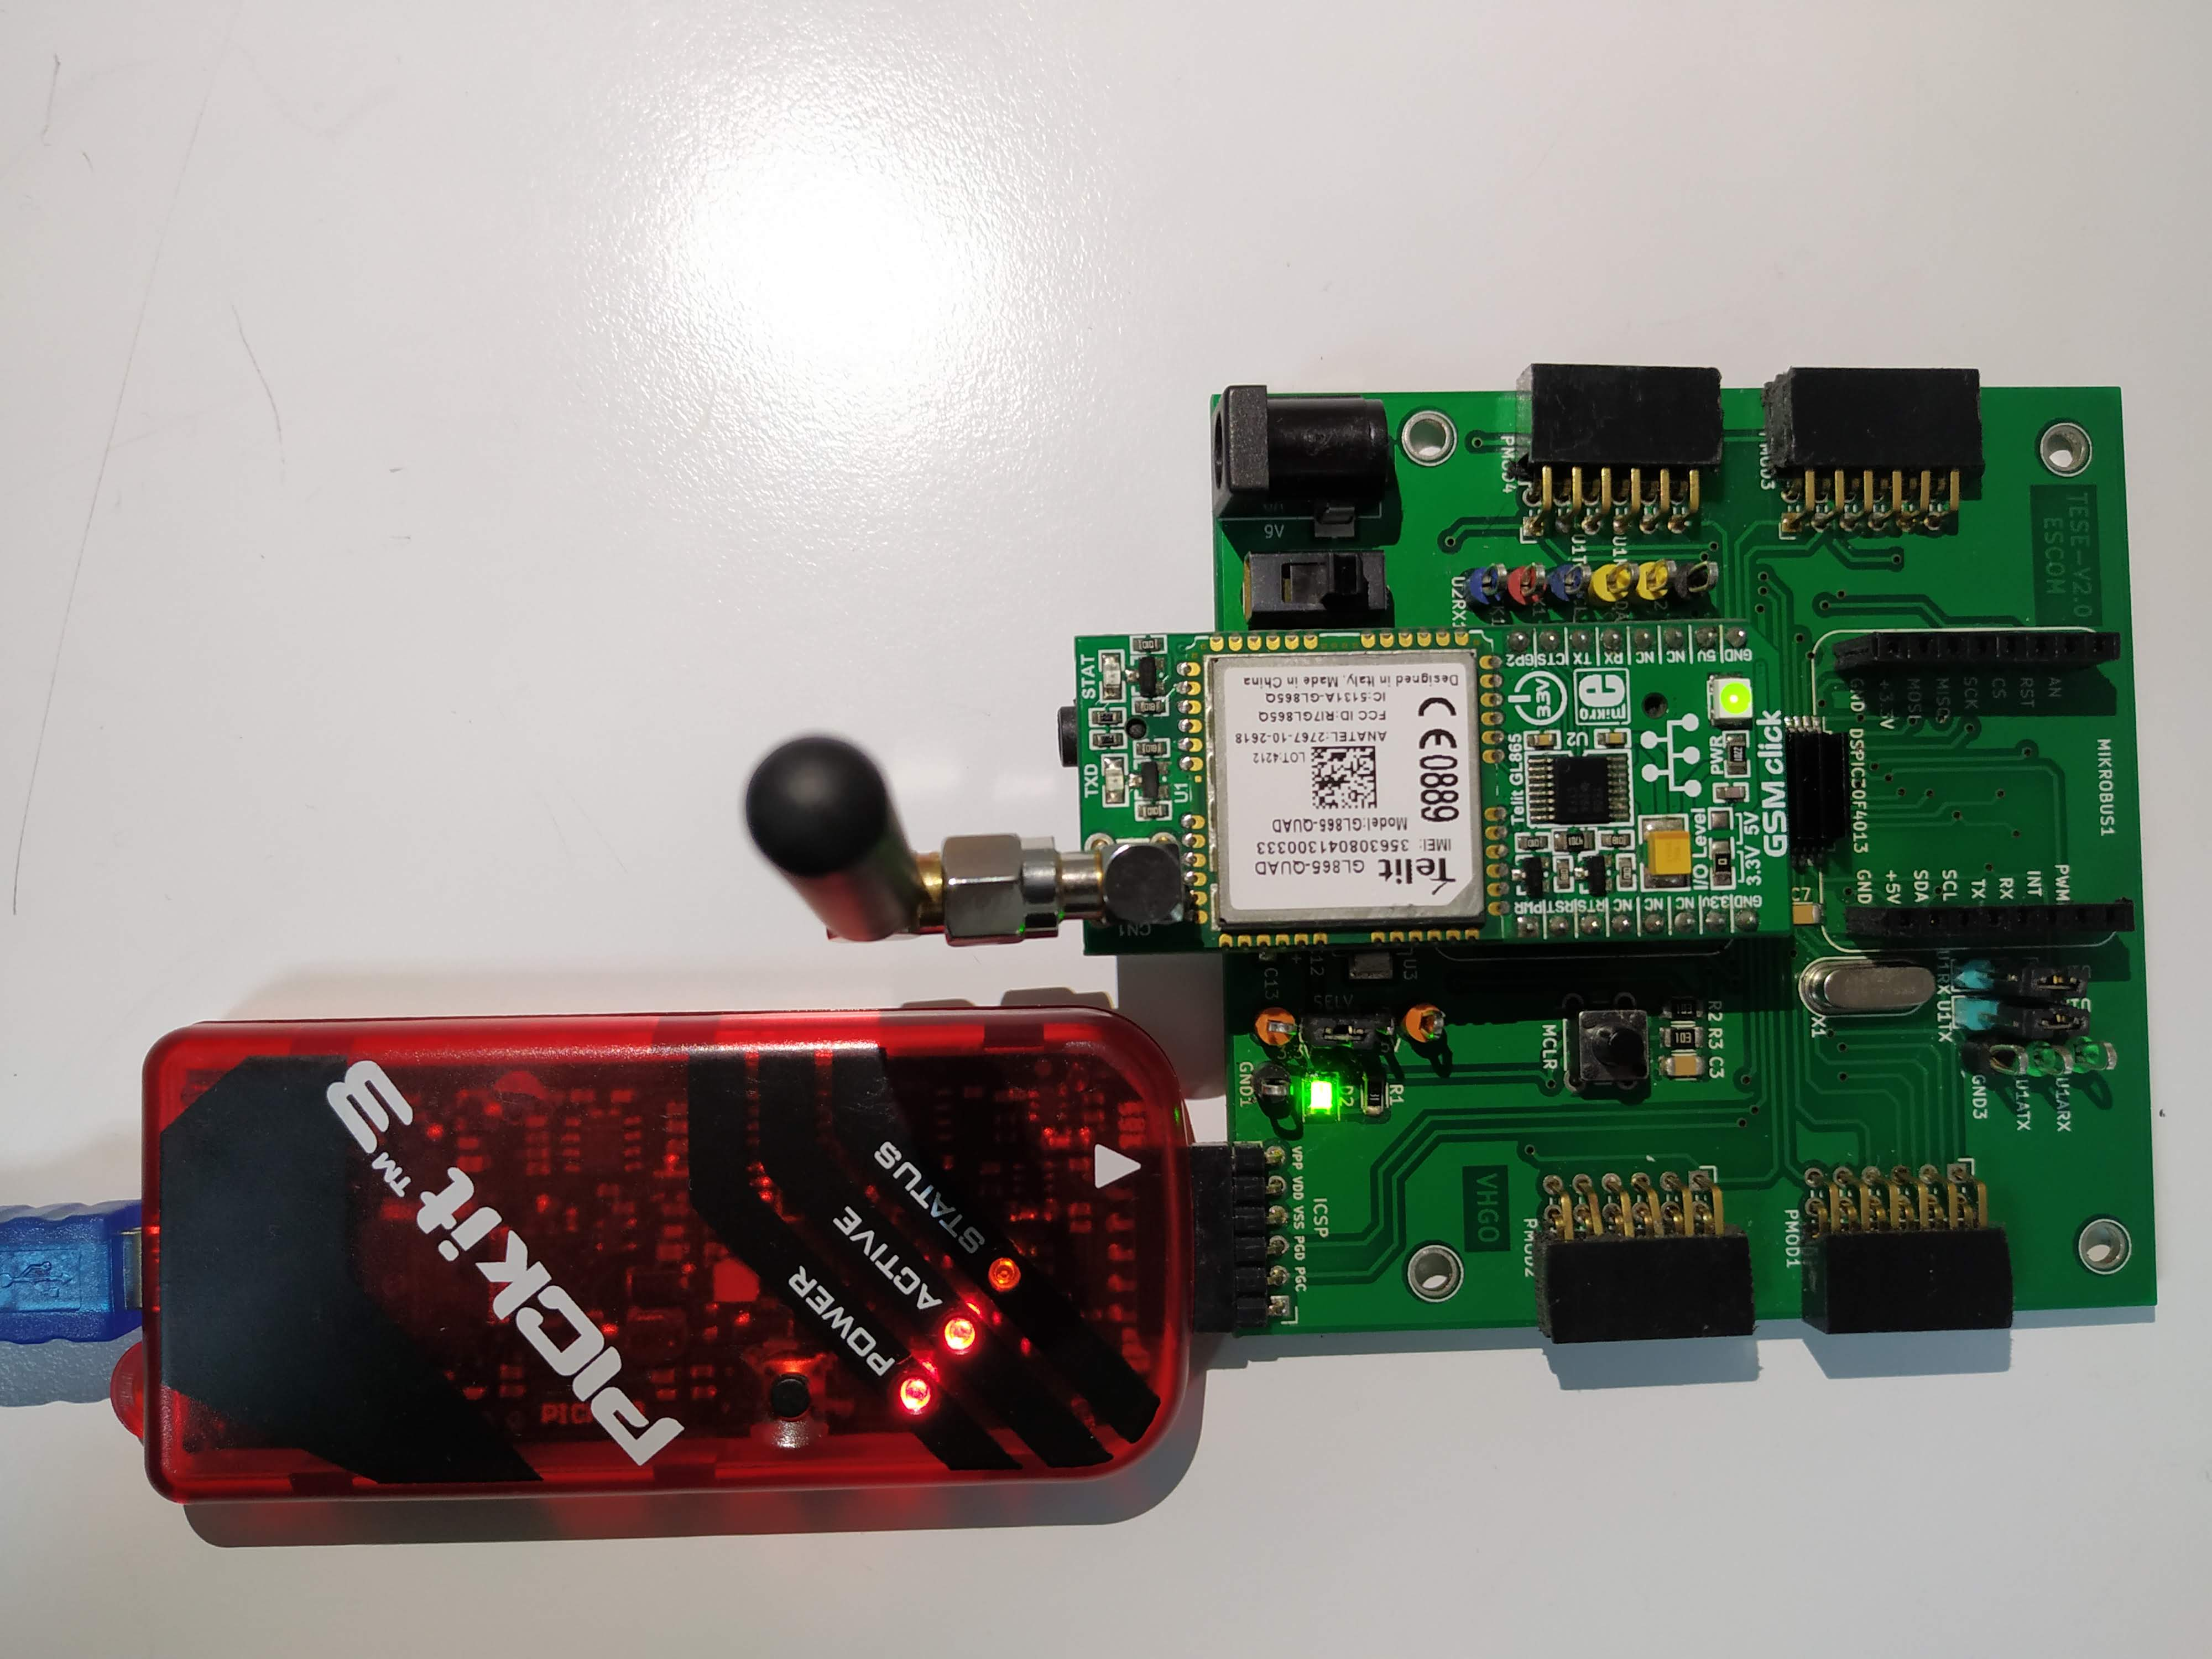
\includegraphics[width=0.7\textwidth]{AvancesPruebas/imagenes/ConexionFisicaGSM.jpg}}
		\caption{Conexión física del módulo GSM con microcontrolador mediante Mikrobus2}
		\label{fig:ConexionFisicaGSM}
	\end{figure}
	
En la figura \ref{fig:RecepcionMsj} se muestra la captura de pantalla que contiene el mensaje recibido en el teléfono celular.

	\begin{figure}[htbp!]
		\centering
		\fbox{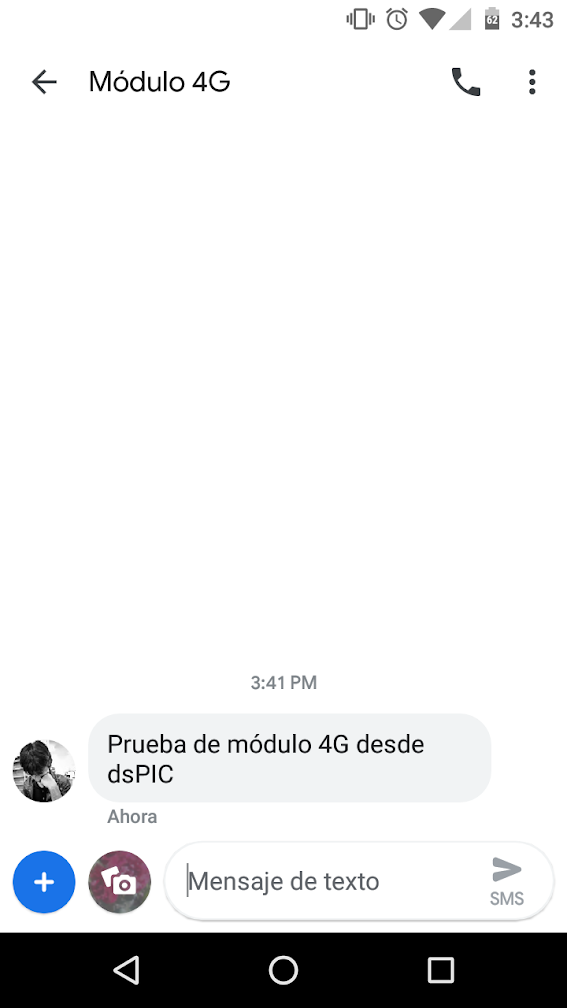
\includegraphics[width=0.35\textwidth]{AvancesPruebas/imagenes/msjModulo.png}}
		\caption{Recepción de mensaje enviado por módulo GSM}
		\label{fig:RecepcionMsj}
	\end{figure}
	
	\clearpage
